% !Mode:: "TeX:UTF-8"
\chapter{基于CS和FA的混合双聚类算法}
元启发式算法在双聚类领域的应用取得了很不错的效果,但元启发式算法本身的缺陷也会影响着双聚类的质量。一般来说,不同的算法有不同的使用范围,一个算法很难做到兼顾全局寻优与快速收敛。比如,布谷鸟算法具有较强的全局搜索能力,而在局部搜索却表现欠佳;萤火虫算法跟布谷鸟算法却刚好相反。全局寻优能力使得算法在寻在双聚类中能够找到更多样的结果,提高了覆盖率;局部寻优能力能够指导算法找到生物意义更加明确的双聚类结果。本文结合布谷鸟算法和萤火虫算法,提出一种混合的元启发式双聚类算法(CS-FA Biclustring,CSFAB),并将CSFAB算法在四个基因表达数据与其他常用的双聚类算法进行了质量验证指标和生物验证指标的比较。

\section{混合双聚类算法分析}
    \subsection{编码设计}
    给定基因表达矩阵$E(X,Y)$,比特串$x_p = (g_1,\dots,g_i,\dots,g_m,s_1,\dots,s_j,\dots,s_n)$,$ p=1,\dots,N, $ 被用来表示一个双聚类或子矩阵$E(I,J)$。其中, $N,m,n$分别是种群数量,$E$的基因数目和样本数目。当$E$中第$i$个基因或第$j$个样本被选为$E(I,J)$时,$g_i=1$或$s_j=1$,否则,$g_i=0$或$s_j=0$,$1\le i \le m$ 且$1\le j \le n$。

    原始的群智能算法的解(粒子,鸟巢,萤火虫)都是多维的连续值,需要映射成对应的比特串后才能用来表示双聚类。通常的做法就是设置上限为1,下限为0,然后判断是否大于0.5,将实数值映射成比特值。如下图所示:
    \begin{figure}[htbp]
        \centering
        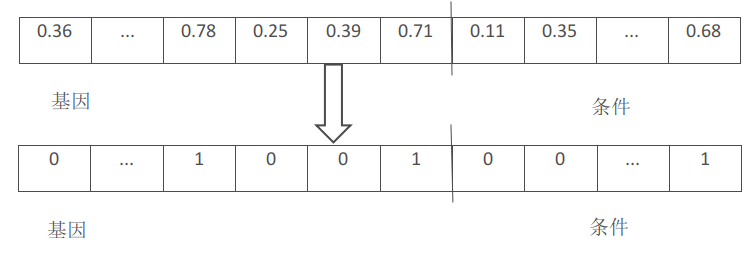
\includegraphics[width = 0.7\textwidth]{coding.png}
        \caption{将连续的解映射为双聚类}
        \label{fig:encoding}
    \end{figure}

    \subsection{适应值函数设计}
    优化算法需要知道优劣的评价标准,在群智能算法中一般称之为适应值。我们需要设计一个适应值函数,用来得到一个解的质量,从而在解与解之间以及算法之间进行比较。正如\ref{section:qualityEval}小节提到的,MSR是最主要也是最直观的质量评价指标,同时双聚类的体积也是衡量好坏的标准之一。一般来说,体积越大的双聚类MSR会相应的变大,而我们希望找到体积大但是MSR较小的双聚类。所以,需要在保持两者之间平衡的同时,能够引导双聚类算法找到更优的解。对于双聚类$B(I,J)$,其适应值为:
    \begin{align}
      f(B) &= MSR(B) + \frac{\lambda}{GV(B)} +\frac{\mu}{CV(B)} + \frac{\omega}{Var(B)}\\
      GV(B) & = |I| \\
      CV(B) & = |J|
    \end{align}
    其中,$GV(B)$,$CV(B)$分别是$B(I,J)$中基因和实验条件的容量。$\lambda,\mu$是针对量纲不同问题,$\lambda,\mu$越大则GV和CV对适应值的影响越大,其值视数据集的情况而定。
    
    \subsection{混合方案设计}
    大致有两种策略将两个算法混合,顺序执行策略和嵌套策略。第一种策略是将一个算法的结果作为另一个算法的输入,特点是两个算法前后互不影响。Nepomuceno 等将SEBI的结果输入到SSB算法中,进一步提高双聚类的质量。第二种策略是将两个算法的揉合到一起,将某一个算法作为局部功能嵌入到另一个算法中,这时两种算法前后不是独立的。例如,Bryan 等将CC算法的局部搜索功能作为SAB算法的一步,以提高双聚类的容量。基于上述二种策略,可有如下三种方案:
    \begin{enumerate}
       \item[(1)] 顺序执行CS-FA:这种方案可以看作将FAB算法的随机初始化替换成CSB算法,先使用CSB算法生成双聚类,然后使用FAB算法进一步提高双聚类的质量,如算法\ref{alg:cs-fa}所示。
        \begin{algorithm}[htbp]
        \caption{CS-FA混合方案} \label{alg:cs-fa}
        % \AlgoBiCaption{这是一个简短的算法中文图题}{This is the English caption of the algorithm}
        \KwIn{$n \times m$的基因表达矩阵E,弃巢比例p,种群大小N,光吸收系数$\gamma$,最大吸引度$\beta_0$,步长因子$\alpha$,最大迭代次数Iter}
        \KwOut{一个满足条件的双聚类B}%
        P = Initialization(E, N) //初始化种群 \\
        $P_{CS}$ = CSB(P,E,p,Iter) \\
        $P_{CS-FA}$ = FAB(P,E,$\gamma$,$\beta_0$,$\alpha$,Iter) \\
        B = Best($P_{CS-FA}$) \\
        return B
        \end{algorithm}

       \item[(2)] 顺序执行FA-CS:与第一种方案刚好相反,将CSB算法的随机初始化改为FAB算法,如算法\ref{alg:fa-cs}所示。
        \begin{algorithm}[htbp]
        \caption{FA-CS混合方案}\label{alg:fa-cs}
        \KwIn{$n \times m$的基因表达矩阵E,弃巢比例p,种群大小N,光吸收系数$\gamma$,最大吸引度$\beta_0$,步长因子$\alpha$,最大迭代次数Iter}
        \KwOut{一个满足条件的双聚类B}%

        P = Initialization(E, N) //初始化种群 \\
        $P_{FA}$ = FAB(P,E,$\gamma$,$\beta_0$,$\alpha$,Iter) \\
        $P_{FA-CS}$ = CSB(P,E,p,Iter) \\
        B = Best($P_{FA-CS}$) \\
        return B \\
        \end{algorithm}
       \item[(3)] 嵌套执行CS-FA
        \begin{algorithm}[htbp]
        \caption{CSFA混合方案}\label{alg:csfa}
        \KwIn{$n \times m$的基因表达矩阵E,弃巢比例p,种群大小N,光吸收系数$\gamma$,最大吸引度$\beta_0$,步长因子$\alpha$,最大迭代次数Iter,最大早熟次数maxEarlyStopCnt}
        \KwOut{一个满足条件的双聚类B}%
        i = 1 \\
        earlyStopCnt = 0 \\
        $B_{old}$ = INF \\
        $P_{fa}$ = Initialization(E, N) //初始化种群 \\
        \Do{(i<=Iter AND earlyStopCnt< maxEarlyStopCnt)}
        {
            $P_{cs}$, $best_{cs}$ = csIter($P_{fa}$, E, p) \\
            $P_{fa}$, $best_{fa}$ = faIter($P_{cs}$, E, $\gamma$,$\beta_0$,$\alpha$) \\
            B = Best( $best_{cs}$, $best_{fa}$) \\
            earlyStopCnt = EarlyStop(earlyStopCnt, B, $B_{old}$)
            $B_{old}$ = B \\
            i++
        }
        return B
        \end{algorithm}
    \end{enumerate}
    \subsection{停止条件}

\section{实验结果及分析}
    \subsection{实验环境}

    \subsection{基因表达数据}

    \subsection{混合方案比较}

    \subsection{CSFAB的质量验证指标比较分析}

    \subsection{CSFAB的生物验证指标比较分析}

\section{本章小结}